\documentclass[letter,11pt]{article}
\usepackage[top=2.0cm, bottom=2.0cm, left=2.0cm, right=2.0cm]{geometry}

% Configuración de Fira Sans para TODO el documento
\usepackage[sfdefault]{FiraSans} % Fuente principal
\usepackage{FiraMono}

\usepackage[utf8]{inputenc}
% Se configura diccionario en español y en entorno de tablas aparecerá el nombre Tabla x
\usepackage[spanish,es-tabla]{babel}
% Se utilizará el punto decimal en lugar de coma para definir números con decimales
\spanishdecimal{.}

% Tablas, imágenes y formato
\usepackage{graphicx}
\usepackage{array}
\usepackage{booktabs}
\usepackage{longtable}
\usepackage{tabularx}
\usepackage{multirow}
\usepackage{multicol}
\usepackage{makecell}
\usepackage{float}
\usepackage{enumitem}
\usepackage{setspace}
\usepackage{fancyhdr}

% Matemáticas y elementos gráficos
\usepackage{amsmath,mathtools,amsfonts,amssymb}
\usepackage{xcolor}
\usepackage{tikz}
\usepackage{tcolorbox}
\usepackage{pdfpages}

% Código y enlaces
\usepackage{listings}
\usepackage{hyperref}

\setlength{\parindent}{0pt}
\setlength{\parskip}{0.55em}
\setlength{\headheight}{22pt}
\setlength{\emergencystretch}{2em}
\graphicspath{{./}}

% Colores institucionales UNAM
\definecolor{unamblue}{RGB}{0,51,102}
\definecolor{unamgold}{RGB}{153,126,48}
\definecolor{myred}{HTML}{911010}
\definecolor{myblue}{HTML}{142966}
\definecolor{myaqua}{HTML}{1EA69A}
\definecolor{backcolour}{rgb}{0.95,0.95,0.92}

\hypersetup{
	colorlinks=false,
	pdfborder={0 0 0},
	pdftitle={Texturizado e Iluminacion - Cempasúchil},
	pdfauthor={Equipo 8}
}

% Estilos de código
\lstdefinestyle{bashstyle}{
	backgroundcolor=\color{backcolour},
	basicstyle=\ttfamily\small,
	numbers=left,
	numberstyle=\tiny\color{gray},
	frame=single,
	tabsize=4,
	breaklines=true,
	captionpos=b,
	keywordstyle=\color{myblue},
	commentstyle=\color{myaqua},
	stringstyle=\color{myred},
	showstringspaces=false,
	columns=fullflexible,
	morekeywords={sudo,apt,git,cmake,open,cd,ls,mkdir,cp}
}
\lstdefinestyle{terminal}{
	backgroundcolor=\color{backcolour},
	basicstyle=\ttfamily\small,
	frame=single,
	tabsize=4,
	breaklines=true,
	showstringspaces=false,
	columns=fullflexible
}

% Recuadro provisional para las capturas
\newcommand{\capturapendiente}[2]{%
	\begin{figure}[H]
		\centering
		\fbox{%
			\parbox[c][5.2cm][c]{0.88\textwidth}{%
				\centering
				\textbf{Captura pendiente}\\[0.3cm]
				\textit{#1}%
			}%
		}
		\caption{#2}
	\end{figure}
}

%% Encabezado y pie de página %%
\pagestyle{fancy}  
\fancyhf{} 
\renewcommand{\headrule}{\hbox to\headwidth{\color{black}\leaders\hrule height \headrulewidth\hfill}}
\renewcommand{\headrulewidth}{0.4pt}
\fancyhead[L]{\color{black}\small{Computación Gráfica e Interacción Humano-Computadora}}
\fancyhead[R]{\color{black}\small{Texturizado e Iluminación}}
\fancyfoot[R]{\small\thepage}

\begin{document}
	\begin{titlepage}
		\thispagestyle{empty}
		\begin{center}
			\vspace{0.8cm}
			\begin{minipage}{0.125\textwidth}
				\centering
				
\includegraphics[width=\textwidth]{UNAM}
			\end{minipage}
			\hfill
			\begin{minipage}{0.7\textwidth}
				\centering
				{\color{black}\fontsize{16}{18}\selectfont
					\textbf{UNIVERSIDAD NACIONAL AUTÓNOMA DE MÉXICO} \\
					\vspace{0.3cm}
					\textbf{FACULTAD DE INGENIERÍA} \\
					\vspace{0.3cm}
					\textbf{COMPUTACIÓN GRÁFICA E INTERACCIÓN HUMANO-COMPUTADORA} \\
					\vspace{0.3cm}
					\textbf{SEMESTRE 2027 - 1}
				}
			\end{minipage}
			\hfill
			\begin{minipage}{0.125\textwidth}
				\centering
				
\includegraphics[width=\textwidth]{UNAM_INGENIERIA}
			\end{minipage}
			
			\vspace{1cm}
			
			\begin{tikzpicture}
				\draw[black, line width=1.5pt] (2\textwidth,0) -- (\textwidth,0);
			\end{tikzpicture}
			
			\vspace{1cm}
			
			{\color{black}\fontsize{18}{20}\selectfont
				\textbf{TEXTURIZADO, COLOR E ILUMINACIÓN} \\
				\vspace{1.5cm}
			}
			
			{\color{black}\fontsize{14}{16}\selectfont
				\begin{tabular}{l r l}
					\textbf{ALUMNOS} & \textit{Basilio Illescas Andrés} & \textit{Product Owner} \\[0.3cm]
					& \textit{Trejo Olvera Emmanuel} & \textit{Scrum Master} \\[0.3cm]
					& \textit{Pérez Olvera Alexis Abraham} & \textit{Developer} \\[0.3cm]
					& \textit{Cruz Macedo Samuel Santiago} & \textit{Developer} \\[0.3cm]
					\textbf{PROFESOR} & \textit{Ing. José Ramón Pérez Athié} & \\[0.3cm]
					\textbf{GRUPO} & \textit{04} & \\[0.3cm]
				\end{tabular}
			}
			
			\vfill
			
			{\color{black}\fontsize{12}{14}\selectfont
				Ciudad Universitaria, CDMX \hfill \today
			}
		\end{center}
	\end{titlepage}
	
	\tableofcontents
	
	\newpage
	
\section{Introducción}
	Tras haber consolidado la base de modelado geométrico en la etapa anterior, el proyecto avanza hacia la aplicación de propiedades ópticas y lumínicas para dotar de realismo a la escena del Día de Muertos. Cabe señalar que la mayoría de los modelos propios fueron remodelados para esta fase, demostrando un mayor compromiso con el proyecto y aumentando significativamente la calidad visual y geométrica de esta entrega.
	
	En esta etapa, los modelos grises son transformados mediante la aplicación de mapas de texturas (Color, Rugosidad y Normales), la configuración de materiales transparentes, la creación de un entorno inmersivo (\textit{Skybox}) y la implementación de un sistema de iluminación dinámica.
	
	El desarrollo se mantuvo en C++17 utilizando OpenGL 3.3. Se programaron \textit{shaders} específicos para procesar texturas PBR simplificadas e iluminar la escena mediante un modelo híbrido que combina la luz ambiental y direccional (Luna) con luces puntuales (cirios y faroles) y atenuación cuadrática. Todo el trabajo fue estructurado para mantener un rendimiento óptimo al procesar miles de instancias texturizadas simultáneamente.
	
	\section{Objetivos}
	\subsection{Objetivo general}
	Implementar un sistema de texturizado, materiales e iluminación en tiempo real sobre la escena previamente modelada, logrando un acabado visual inmersivo que respete las proporciones geométricas y optimice los recursos en un entorno multiplataforma.
	
	\subsection{Objetivos específicos}
	\begin{itemize}[leftmargin=*]
		\item Diseñar y hornear texturas PBR (Color, Normales y Rugosidad) a partir de nodos procedurales en Blender.
		\item Implementar la carga dinámica de imágenes 2D con ImageIO en macOS y \texttt{stb\_image} en Windows y Linux.
		\item Configurar un \textit{Skybox} con texturas panorámicas para simular la transición lumínica del atardecer.
		\item Desarrollar \textit{shaders} que calculen luces puntuales con atenuación y refracción óptica simulada para vidrios y líquidos.
		\item Garantizar la correcta compilación y ejecución en macOS, Windows y distribuciones Linux con soporte para OpenGL 3.3.
	\end{itemize}
	
	\section{Alcance de la entrega}
	El alcance de esta fase comprende el texturizado de los modelos propios de la ofrenda y el entorno, la aplicación de materiales a los modelos de librería, la creación procedural de coordenadas UV, el mapeo de transparencias (recorte alfa) y la programación de los \textit{shaders} de iluminación.
	
	Se incluyen los mapas difusos, mapas de normales calculados en tiempo real mediante derivadas matemáticas de los fragmentos, canales de metalidad/rugosidad y el entorno atmosférico cúbico. También se incorpora la refracción óptica simulada a través de cálculos de transmitancia y \textit{Fresnel} para jarrones y vasos.
	
	Quedan fuera de esta entrega las animaciones esqueléticas complejas, las sombras dinámicas de alta resolución (\textit{Shadow Mapping}) y las reflexiones especulares en tiempo real basadas en trazado de rayos.
	
	\section{Metodología de trabajo ágil}
	Para la administración de esta segunda etapa del proyecto, el equipo continuó iterando sobre el marco de trabajo \textit{Scrum}, adaptando los \textit{sprints} a las necesidades específicas de mapeo UV, programación de \textit{shaders} y pruebas de rendimiento.
	
	El \textit{Product Backlog} se reestructuró enfocándose en el acabado visual y la optimización. El desarrollo se dividió en cuatro iteraciones principales (\textit{sprints}):
	\begin{enumerate}[leftmargin=*]
		\item \textbf{Definición y Diseño Procedural:} Asignación de propiedades de materiales, creación de redes nodales en Blender y horneado (\textit{baking}) de texturas PBR.
		\item \textbf{Programación Gráfica:} Desarrollo e integración de \textit{shaders} para iluminación híbrida, cálculos de normales en tiempo real y transmisión óptica.
		\item \textbf{Integración y Pruebas Multiplataforma:} Creación de rutinas nativas para carga de imágenes, validación del \textit{Skybox} y resolución de conflictos de despliegue en macOS, Linux y Windows.
		\item \textbf{Optimización y Refactorización:} Identificación de cuellos de botella lumínicos, retopología geométrica de modelos excedidos en polígonos y automatización mediante los lanzadores nativos.
	\end{enumerate}
	
	Las reuniones de sincronización asíncronas permitieron identificar tempranamente los bloqueos arquitectónicos (como los conflictos del repositorio en Git por configuraciones específicas de SO), facilitando una toma de decisiones rápida por parte del \textit{Scrum Master} y los desarrolladores para unificar el \texttt{CMakeLists.txt} y mantener la entrega en los plazos establecidos.
	
	\section{Diseño y desarrollo}
	
	\subsection{Flujo de Trabajo en Blender: Texturas Procedurales}
	Para garantizar una alta calidad visual sin depender de fotografías externas, se optó por un flujo de trabajo procedural. Las texturas de los modelos propios fueron diseñadas directamente en el editor de nodos de Blender mediante funciones matemáticas de ruido y mezcla de colores.
	
	Posteriormente, estas redes nodales complejas fueron horneadas (\textit{baked}) a mapas de bits tradicionales (Color, Rugosidad y Normales). Finalmente, los modelos, junto con sus texturas, fueron exportados bajo el estándar glTF 2.0 y almacenados en la ruta \texttt{assets/models/propios/}. Este empaquetado aseguró una lectura eficiente al cargar la escena en OpenGL.
	
	\subsection{Mapeo de Normales y Materiales PBR}
	En lugar de cargar y precalcular los vectores tangentes en los vértices, el \textit{fragment shader} (\texttt{escena.frag}) calcula las normales mapeadas en tiempo real. Esto se logró utilizando las funciones \texttt{dFdx} y \texttt{dFdy} sobre la posición de los vértices y las coordenadas UV, permitiendo extraer relieves altamente detallados para elementos como el pan de muerto, los muros de adobe y las calaveritas de azúcar de manera muy optimizada.
	
	\subsection{Generación Procedural de UVs y Recorte Alfa}
	Para el empedrado y la alfombra de cempasúchil, las coordenadas UV se generaron de forma procedural en el archivo \texttt{Camino.cpp} basándose en la longitud de arco de la spline Catmull-Rom. El \textit{shader} procesa máscaras con recortes alfa (\texttt{uCorteAlfa}) para dar forma a los bordes dentados del papel picado y descartar los píxeles transparentes de los pétalos dispersos, reduciendo drásticamente la carga geométrica.
	
	Para evitar la superposición o penetración geométrica de texturas complejas, se implementó una cuadrícula espacial de alturas en la clase \texttt{ApoyoDulce} (\texttt{ApoyoDulces.h}), la cual recorta cada triángulo contra la celda correspondiente garantizando un apilamiento perfecto y natural de los elementos.
	
	\subsection{Iluminación Híbrida y Transmisión}
	El modelo lumínico abandonó la luz direccional genérica de la fase de modelado por un sistema híbrido. Éste consiste en:
	\begin{itemize}[leftmargin=*]
		\item \textbf{Luz direccional lunar:} Un tinte direccional tenue modificado con parámetros de oclusión ambiental.
		\item \textbf{Luces puntuales:} Un arreglo en el \textit{shader} que soporta hasta 64 fuentes simultáneas (aplicado a cirios y veladoras) con atenuación cuadrática en base a un radio fijo.
		\item \textbf{Transmisión óptica:} Un cálculo aproximado sin refracción de pantalla utilizando el índice de refracción (\texttt{uIor}) y el cálculo de \textit{Fresnel} para dotar de realismo a objetos de vidrio y agua, reforzando cantos y permitiendo visibilidad hacia atrás sin artefactos.
	\end{itemize}
	
	\subsection{Entorno Atmosférico (Skybox)}
	Se integró un mapa cúbico para el cielo mediante la clase \texttt{Skybox}. El \textit{vertex shader} del cielo elimina la traslación de la matriz de vista asegurando que el horizonte permanezca estático a medida que el jugador se mueve. En el \textit{fragment shader} (\texttt{cielo.frag}), se extrae la luminancia del píxel (\textit{luma}) para oscurecer dinámicamente el atardecer original y mezclarlo hacia una tonalidad nocturna inmersiva.
	
	\section{Retos arquitectónicos y compatibilidad multiplataforma}
	La validación se realizó en macOS, Windows y Linux. Además de los problemas visuales, se probaron la configuración con CMake, los compiladores, la localización de recursos y los lanzadores sin consola. Los incidentes relevantes y su solución final fueron los siguientes:
	
	\begin{enumerate}[leftmargin=*]
		\item \textbf{Artefactos generados y divergencias en Git.}
		Los productos de CMake, Xcode y Visual Studio no son portables entre equipos. Se amplió \texttt{.gitignore} para excluir \texttt{build-*}, cachés, binarios, objetos, bibliotecas, registros y archivos propios del sistema operativo. La documentación y el código fuente permanecen versionados; las ramas divergentes se integraron mediante \texttt{git pull --rebase} para conservar tanto la documentación remota como las correcciones locales.

		\item \textbf{Tamaño del \textit{framebuffer} en pantallas de alta resolución.}
		En Retina y otras pantallas con escalado, las dimensiones lógicas de la ventana no coinciden con los píxeles renderizables. Se empleó \texttt{glfwGetFramebufferSize} antes de \texttt{glViewport}, evitando que la escena ocupara sólo una fracción de la ventana.

		\item \textbf{Localización portable de recursos.}
		La aplicación no debe depender del directorio desde el que fue invocada. \texttt{Rutas.cpp} obtiene la ubicación real del ejecutable con \texttt{GetModuleFileNameW} en Windows y \texttt{/proc/self/exe} en Linux; después busca \texttt{assets/} y \texttt{shaders/} con \texttt{std::filesystem}. En Windows se usan rutas anchas para admitir caracteres UTF--8. Esto eliminó dependencias de separadores y directorios de trabajo específicos.

		\item \textbf{Texturas visibles en macOS, pero ausentes en Windows y Linux.}
		La primera versión de \path{ImageLoader.cpp} sólo implementaba la decodificación bajo \texttt{\#ifdef} \texttt{\_\_APPLE\_\_}; en las demás plataformas devolvía \texttt{false}. La geometría y los colores planos aparecían, pero fallaban PNG, JPEG y el \textit{skybox}. La solución fue conservar ImageIO/CoreGraphics en macOS e integrar \texttt{stb\_image} 2.30 para Windows y Linux. La cabecera se incluyó en \path{external/stb/} y se limitaron los decodificadores a PNG y JPEG. La despremultiplicación alfa de CoreGraphics se mantuvo para evitar bordes oscuros en macOS.

		\item \textbf{Lanzador de macOS.}
		Usar directamente un script como \path{CFBundleExecutable} produjo fallos de apertura y resultados afectados por la caché de Finder. El paquete final utiliza un pequeño lanzador Mach--O nativo que localiza el proyecto y delega la compilación a \path{Contents/Resources/iniciar.zsh}. La aplicación permanece local y sin firma, por lo que la primera apertura puede requerir clic derecho, \textbf{Abrir}. Los detalles se guardan en \path{logs/lanzador-macos.log}.

		\item \textbf{VBScript, PowerShell y Visual Studio en Windows.}
		La cadena que invocaba PowerShell desde VBScript quedó inicialmente sin terminar; se corrigió construyendo las comillas con \texttt{Chr(34)}. Después, el lanzador buscaba exclusivamente Visual Studio 2022 aunque el equipo de prueba tenía Visual Studio 2026. Ahora consulta \texttt{vswhere.exe}, selecciona automáticamente \texttt{Visual Studio 17 2022} o \texttt{Visual Studio 18 2026} y usa carpetas de compilación separadas.

		\item \textbf{Diagnósticos incompletos y compilaciones simultáneas en Windows.}
		Con \texttt{ErrorActionPreference} configurado como \texttt{Stop}, Windows PowerShell interpretaba la primera línea de \texttt{stderr} de CMake como excepción y truncaba el diagnóstico. Se encapsularon las llamadas nativas para registrar toda la salida y evaluar \texttt{LASTEXITCODE}. Además, un doble clic durante una compilación oculta iniciaba otro MSBuild y causaba \textit{Permission denied} sobre archivos \texttt{.obj}; un \textit{mutex} nombrado impide ejecuciones concurrentes.

		\item \textbf{Diferencias de compilador y coma flotante.}
		MSVC no aceptó el uso indirecto de \texttt{std::array}; se agregó explícitamente \texttt{<array>}. También se observaron 3055 instancias en Windows frente a una referencia de 3057 en macOS por diferencias de redondeo en pruebas geométricas con \texttt{float}. Una variación pequeña ahora se registra como aviso y una desviación mayor continúa deteniendo la carga, de modo que no se ocultan errores reales.

		\item \textbf{OpenGL 3.3 dentro de una máquina virtual.}
		Windows 11 ARM bajo UTM compiló correctamente, pero su controlador VirtIO 3D expuso aceleración DirectX y no un contexto OpenGL 3.3 compatible. La aplicación falló al crear la ventana, mientras que el mismo repositorio funcionó en Windows físico con el controlador oficial de la GPU. Por tanto, la compilación dentro de una VM no garantiza el nivel de OpenGL requerido; debe verificarse la capacidad gráfica del entorno invitado.
	\end{enumerate}
	
	\section{Estructura del proyecto}
	El proyecto incorpora nuevos archivos y carpetas destinados a la administración de las texturas y los \textit{shaders} actualizados. Notarás que la columna de Elementos se ha ampliado para mayor claridad.
	
	\begin{longtable}{>{\ttfamily}p{6.0cm}p{9.0cm}}
		\caption{Archivos y carpetas nuevos o actualizados.}\label{tab:estructura_nueva}\\
		\toprule \normalfont Elemento & \normalfont Propósito\\ \midrule \endfirsthead
		\toprule \normalfont Elemento & \normalfont Propósito\\ \midrule \endhead
		src/render/Skybox.cpp & Carga del mapa cúbico, manipulación del \textit{luma} y renderizado esférico del cielo.\\
		src/render/ImageLoader.cpp & Decodificación PNG/JPEG mediante ImageIO en macOS y \texttt{stb\_image} en Windows/Linux.\\
		src/Rutas.cpp & Localización del ejecutable y resolución portable de \texttt{assets/} y \texttt{shaders/}.\\
		src/render/Shader.cpp & Analizador sintáctico para inyección de macros (\texttt{\#define}) y compilación dinámica de GLSL.\\
		shaders/escena.frag & Algoritmos de iluminación, derivadas parciales para relieves, transmitancia y variables PBR.\\
		shaders/escena.vert & Transformación espacial adaptada para procesamiento de instancias texturizadas y tintes de color.\\
		assets/textures/ & Texturas base, mapas de color, metalidad/rugosidad generados procedimentalmente.\\
		assets/skybox/atardecer/ & Fragmentos de la imagen esférica para procesar el entorno panorámico de la escena.\\
		external/stb/stb\_image.h & Decodificador de imágenes de un solo encabezado incluido para Windows y Linux.\\
		ejecutables/ & Lanzadores y scripts silenciosos para macOS, Windows y Linux.\\
		\bottomrule
	\end{longtable}
	
	\section{Capturas de la aplicación}
	
	\begin{figure}[H]
		\centering
		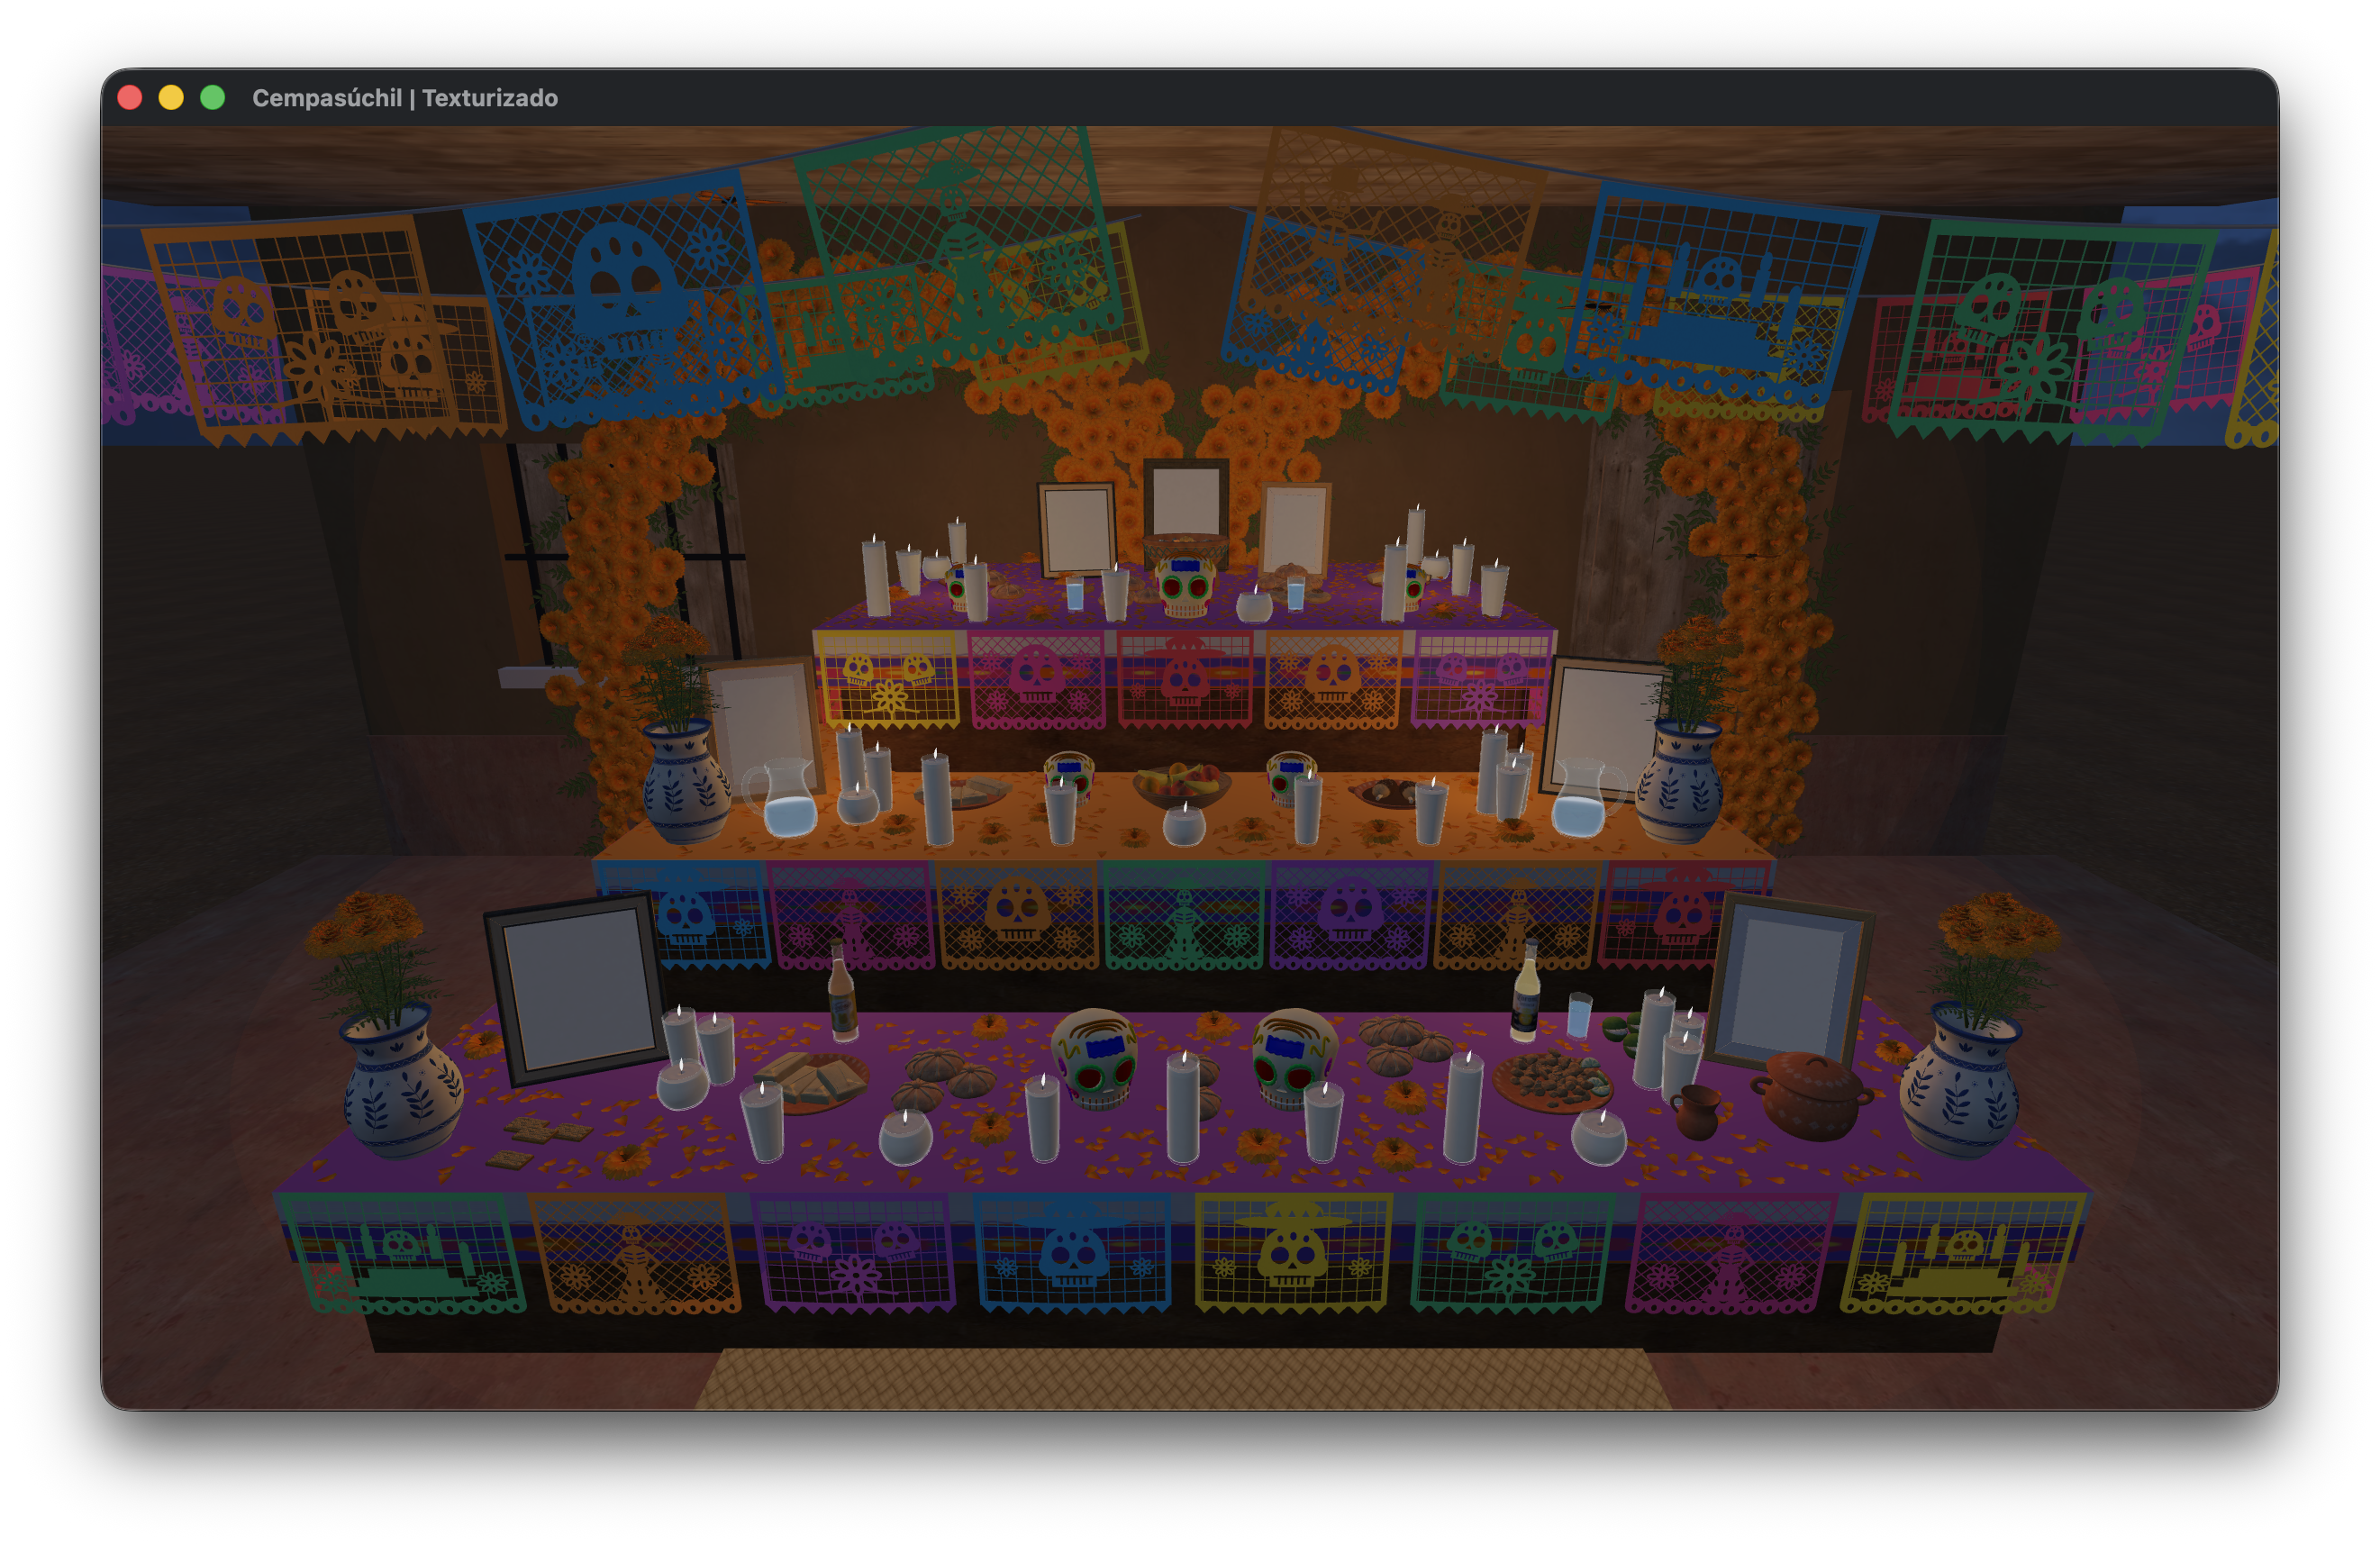
\includegraphics[width=0.85\textwidth]{images/vista-general-ofrenda.png}
		\caption{Vista general de la ofrenda iluminada.}
	\end{figure}
	
	\begin{figure}[H]
		\centering
		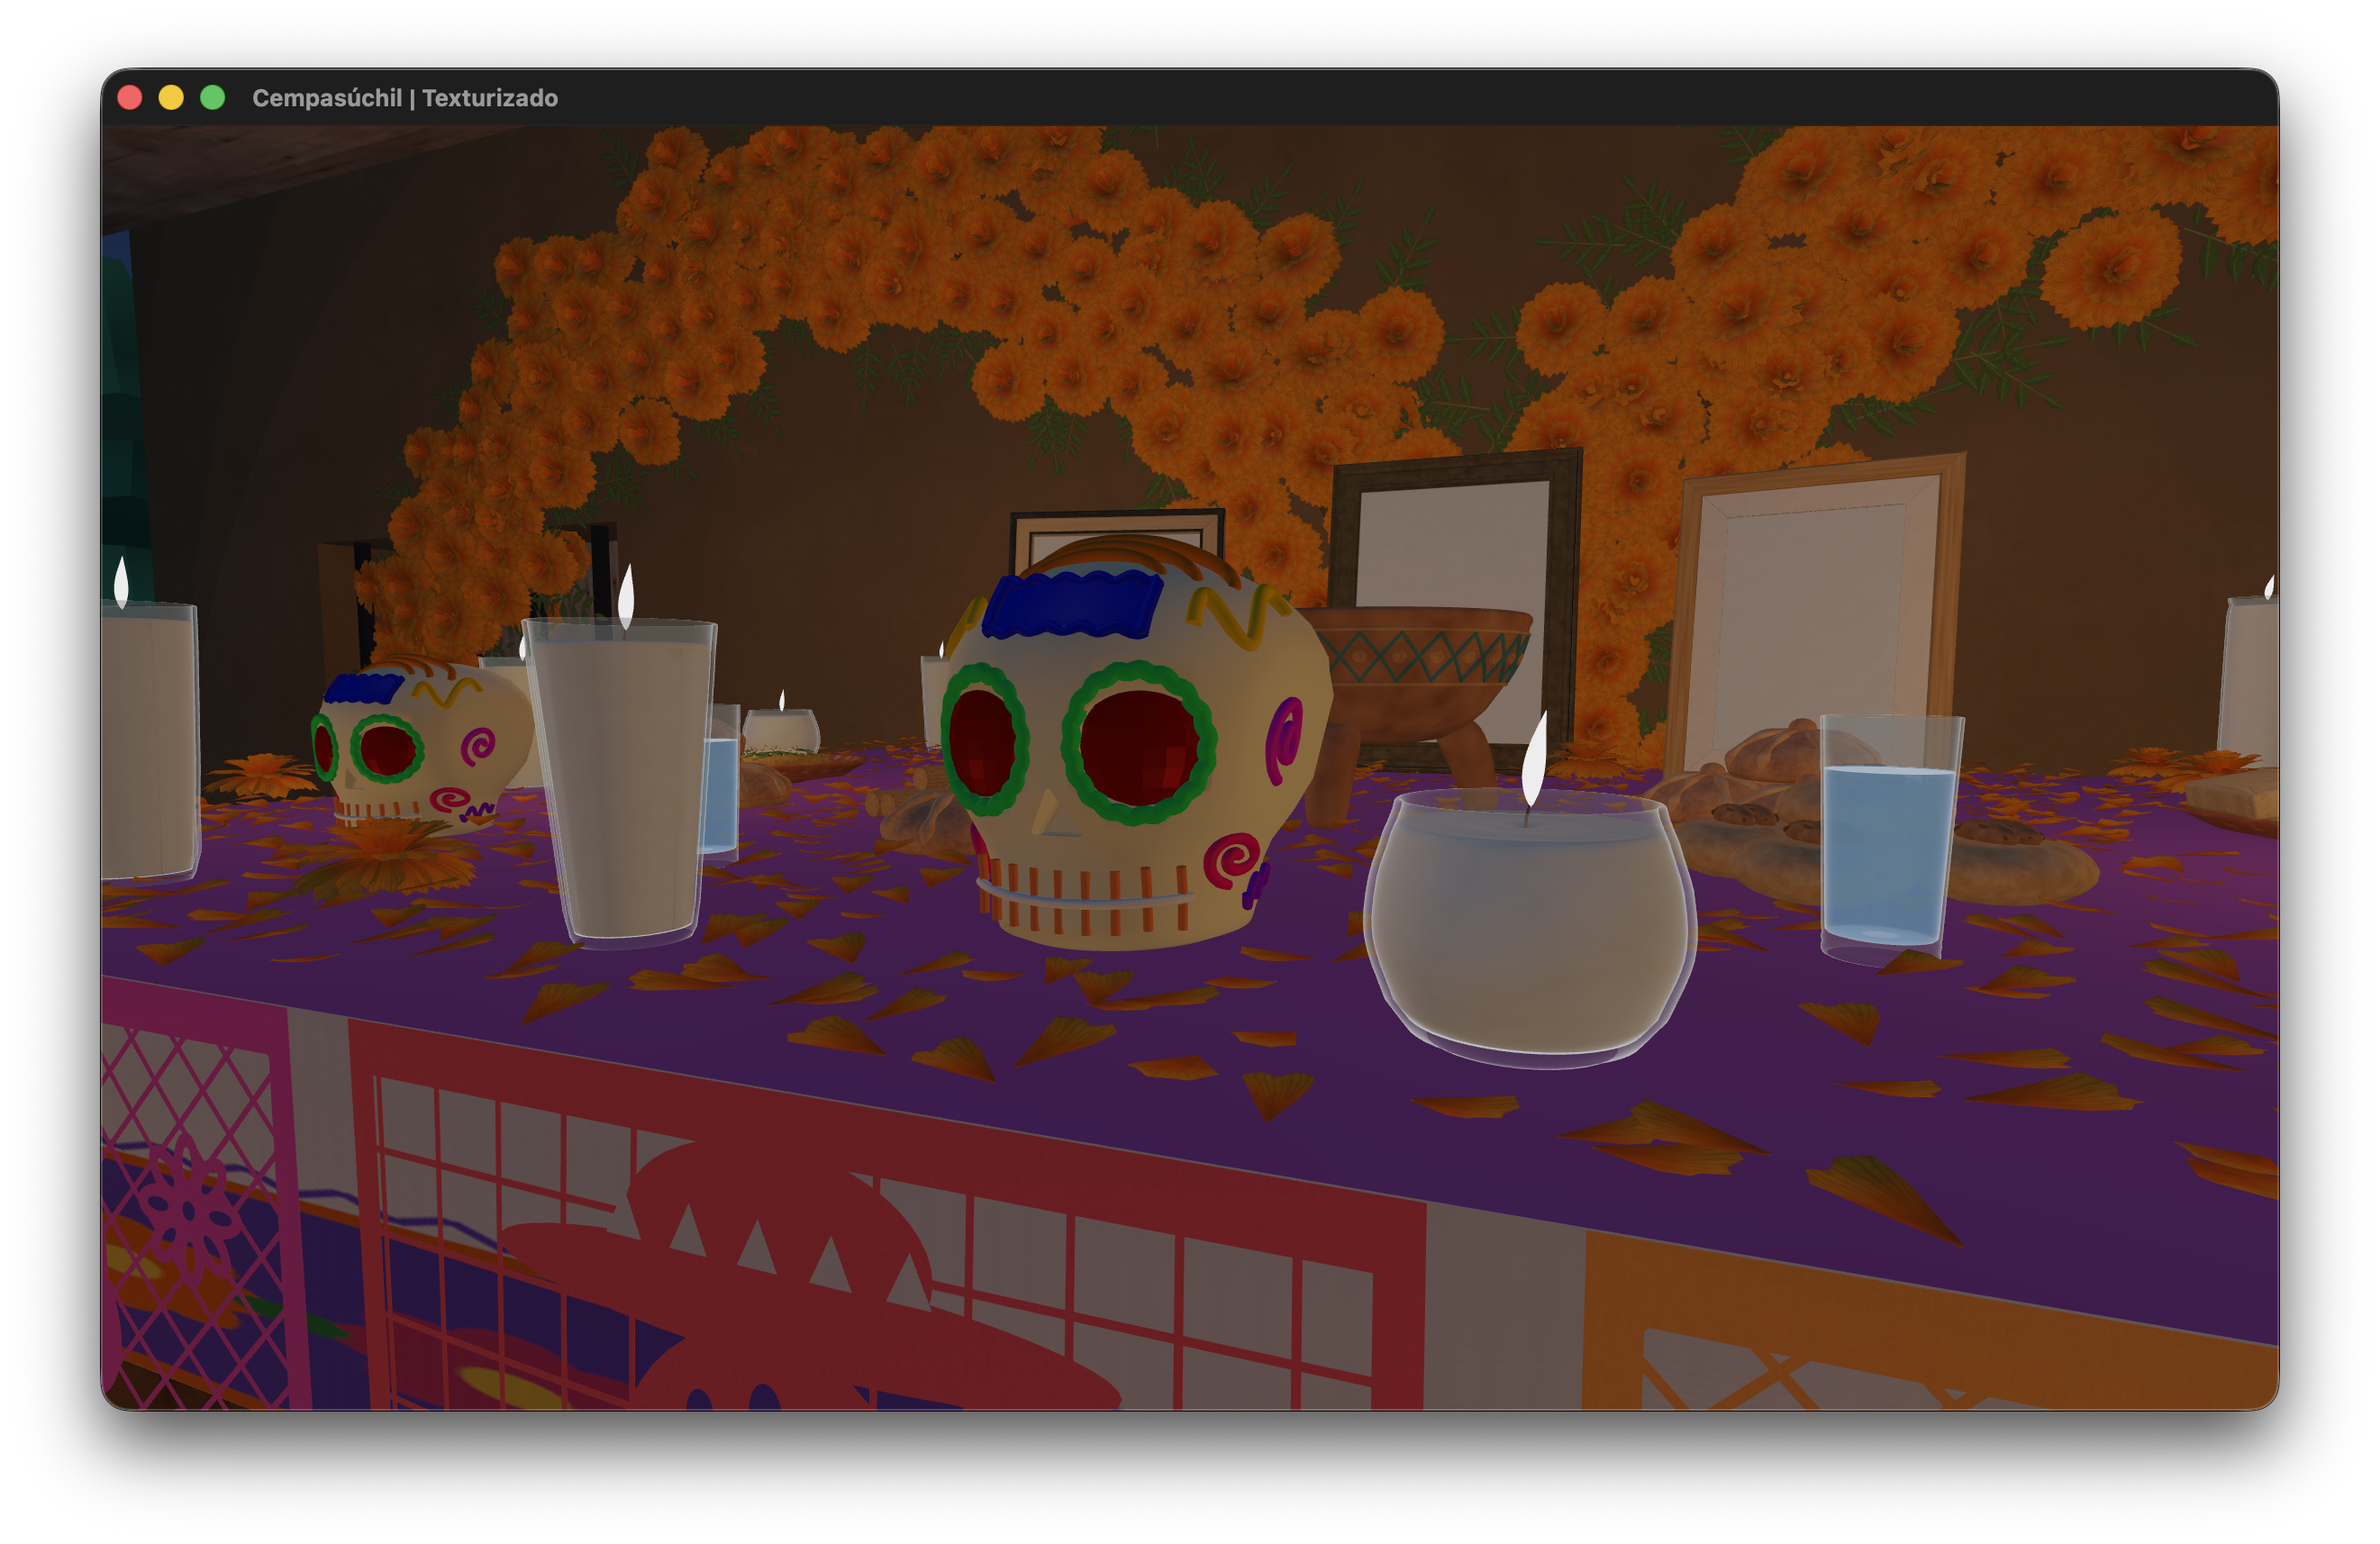
\includegraphics[width=0.85\textwidth]{images/detalle-PBR.png}
		\caption{Detalle de las texturas PBR y efecto de luz puntual sobre los objetos.}
	\end{figure}
	
	\begin{figure}[H]
		\centering
		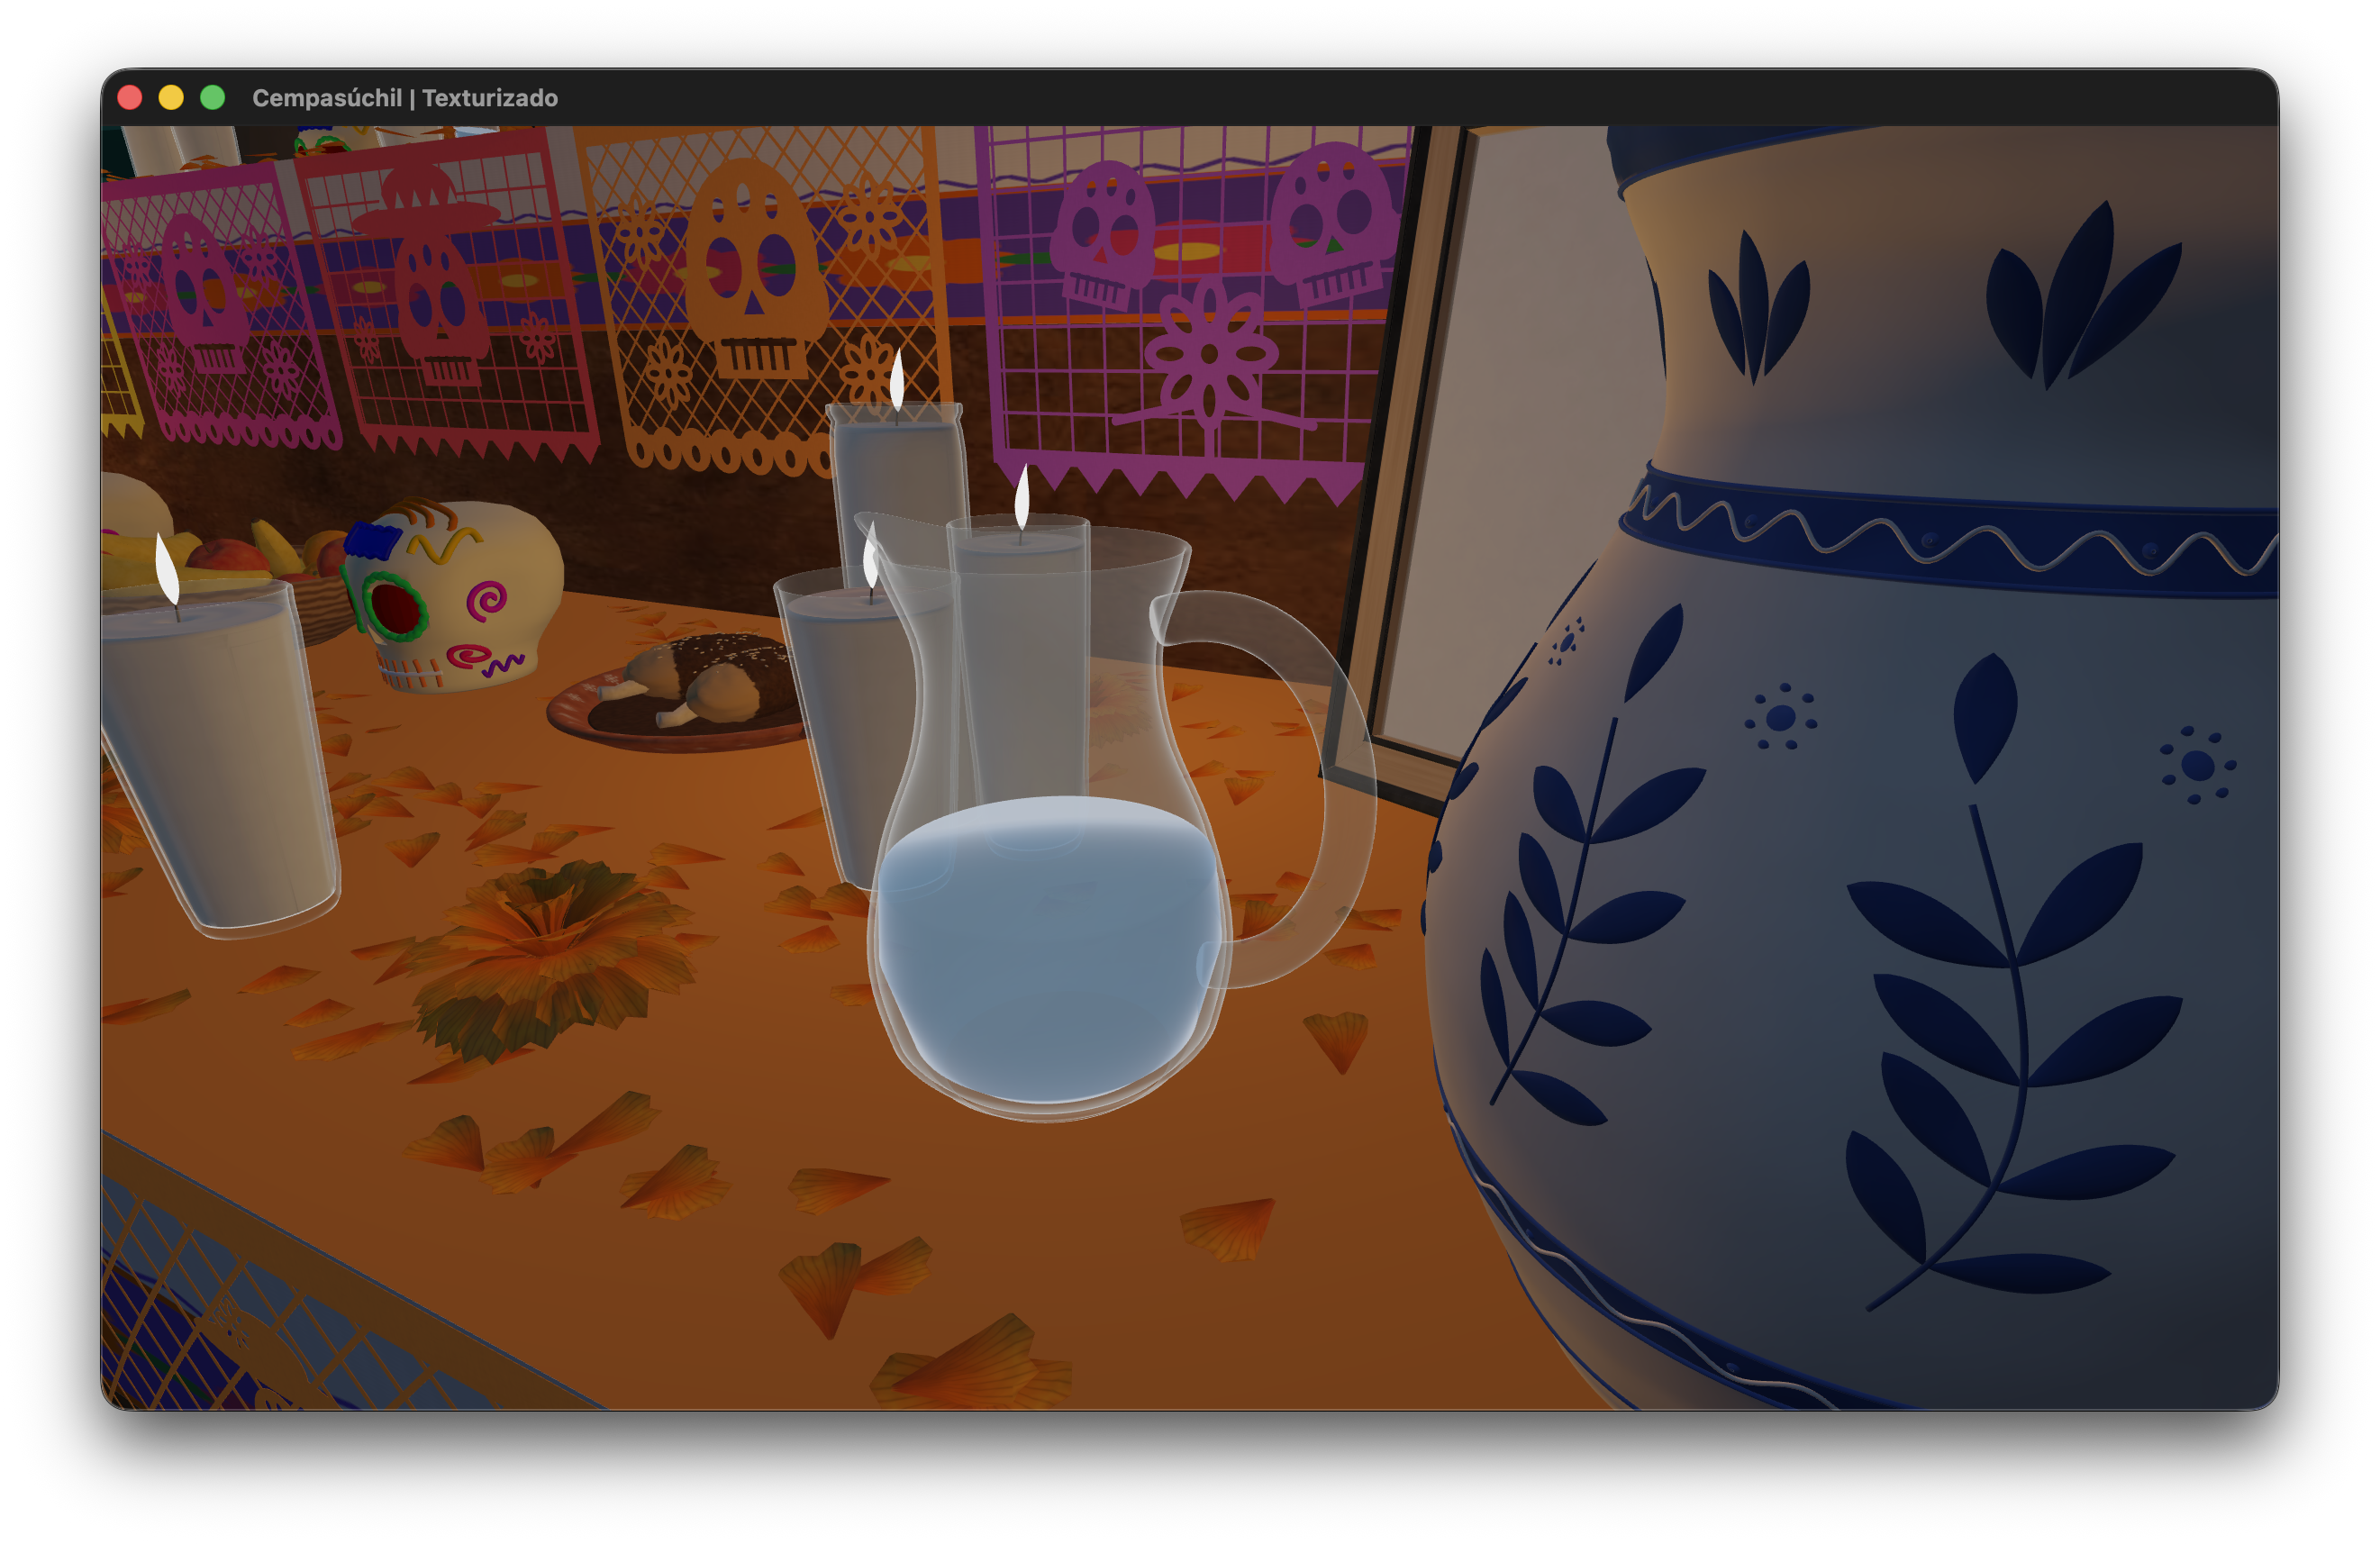
\includegraphics[width=0.85\textwidth]{images/fresnel-1.png}
		\caption{Aproximación óptica en materiales de vidrio y líquidos.}
	\end{figure}
	
	\begin{figure}[H]
		\centering
		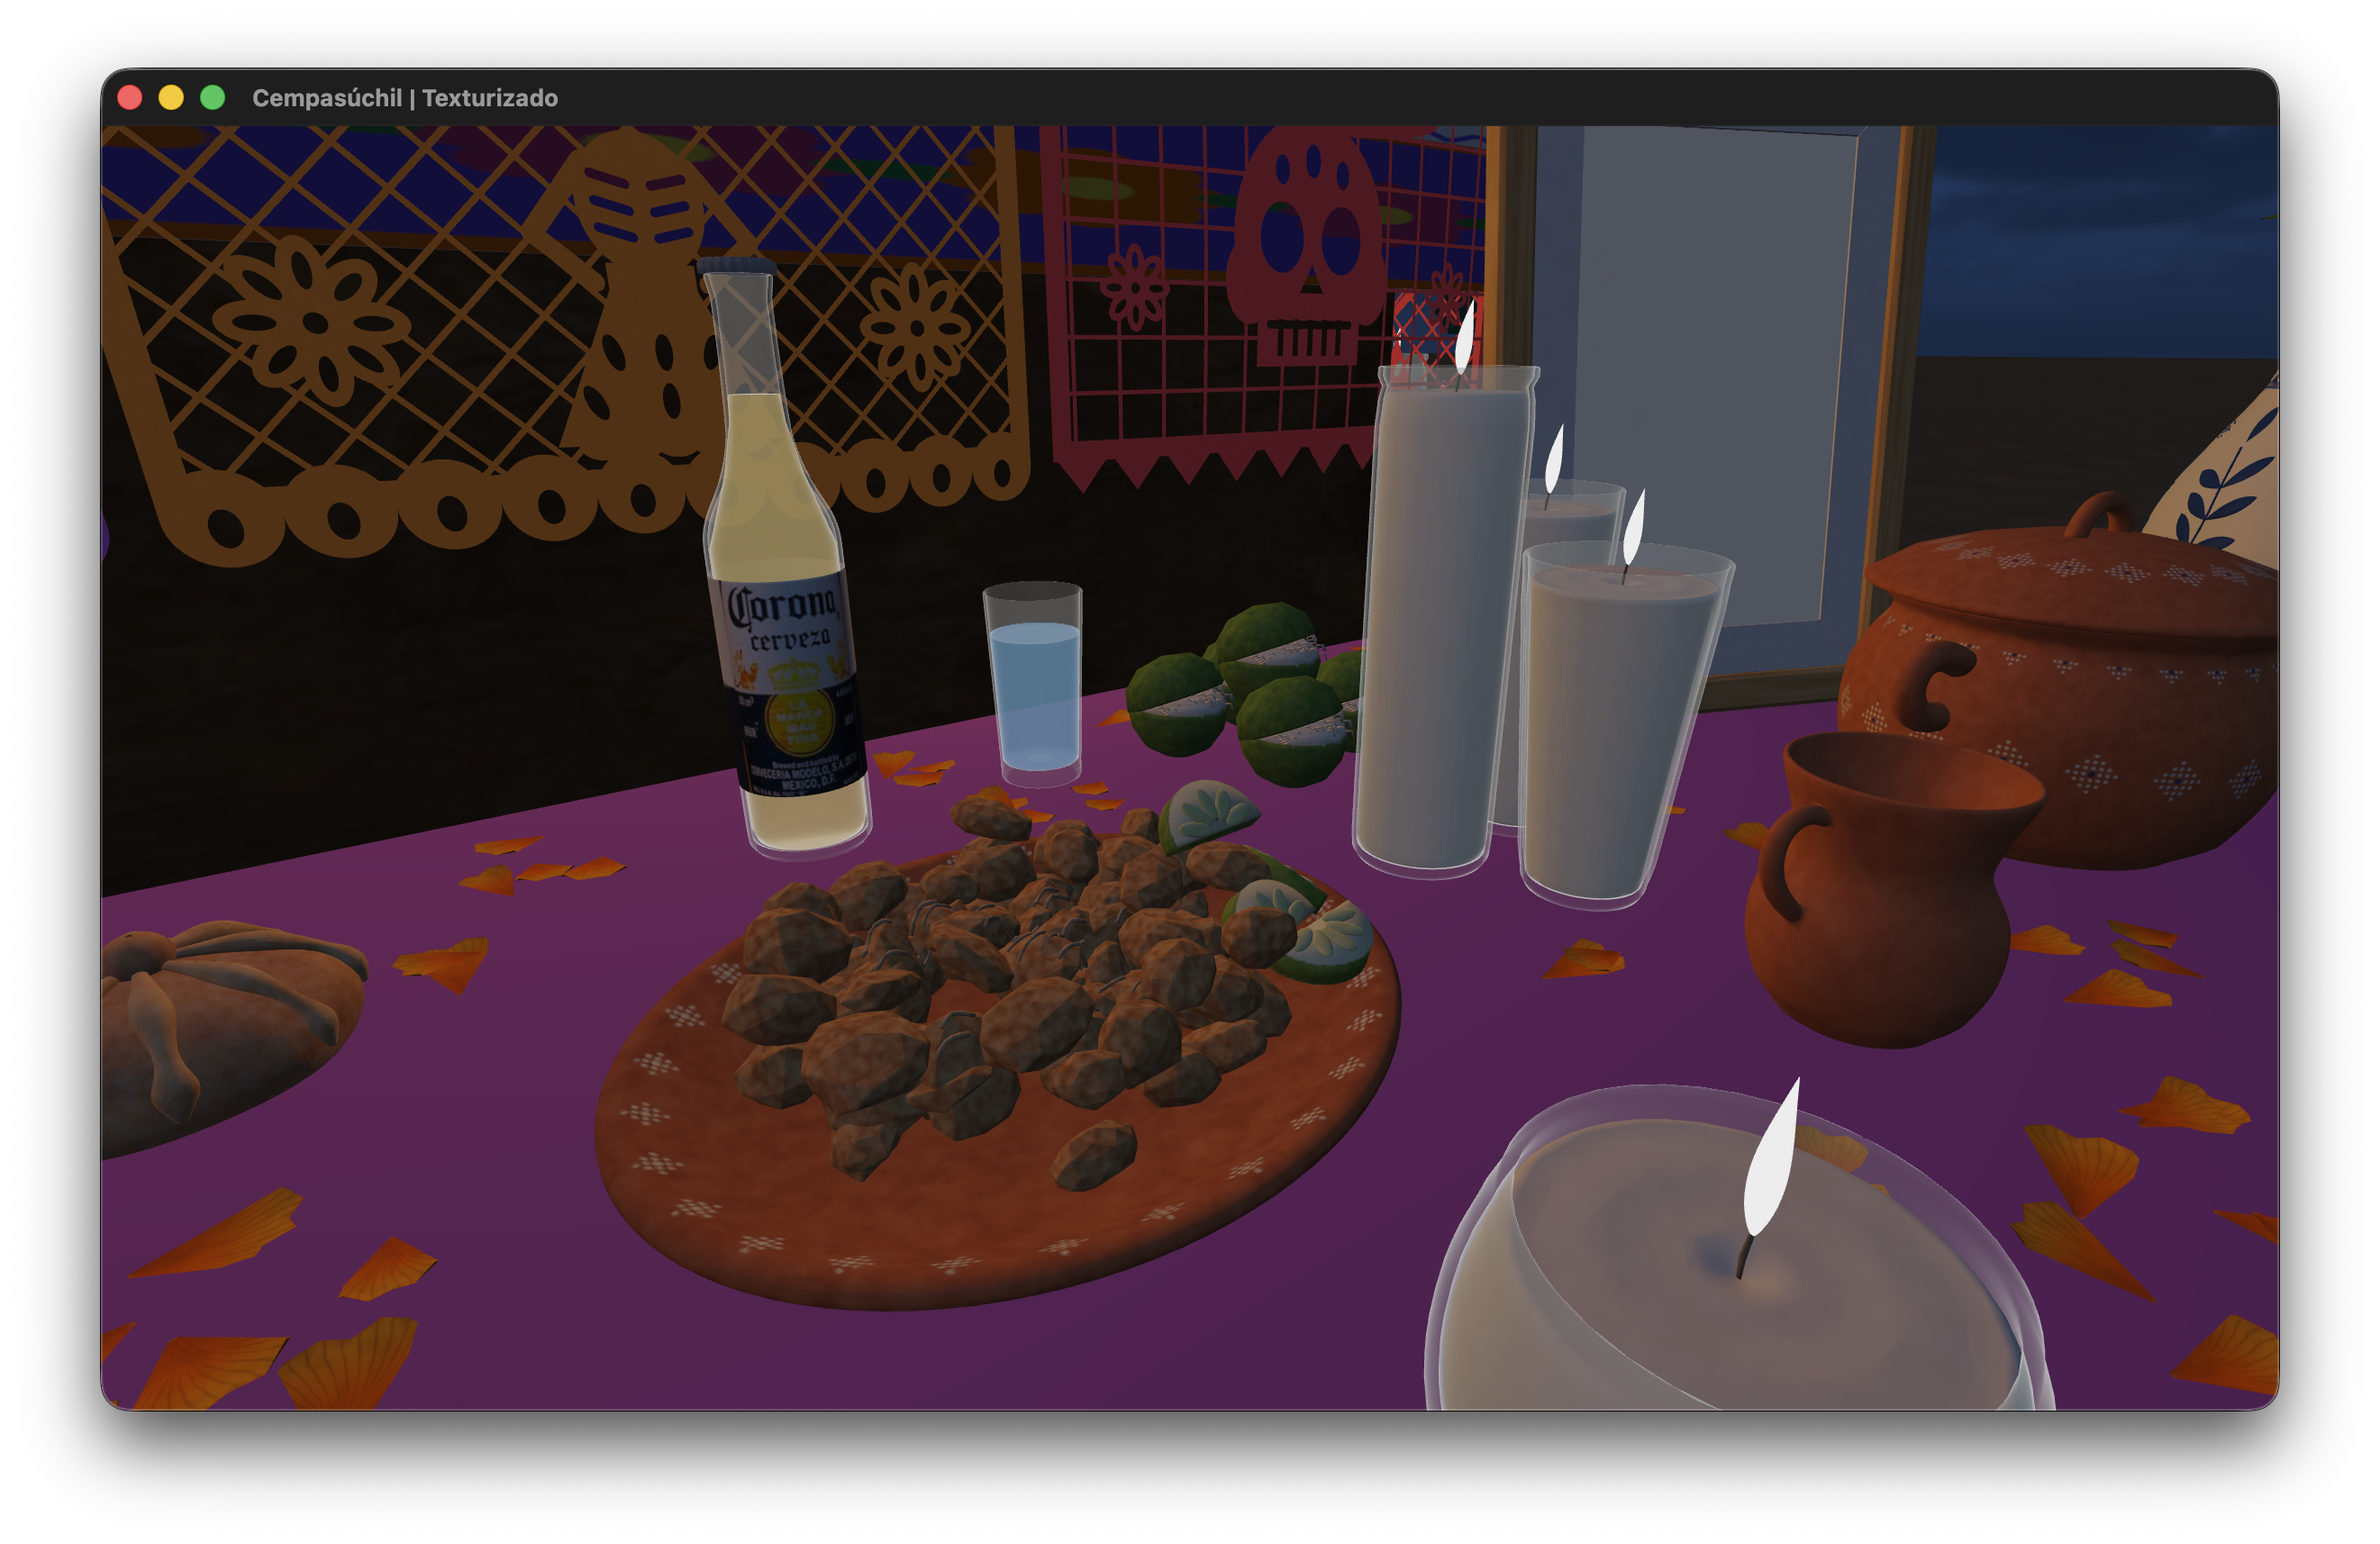
\includegraphics[width=0.85\textwidth]{images/fresnel-2.png}
		\caption{Aproximación óptica en materiales de vidrio y líquidos.}
	\end{figure}
	
	\begin{figure}[H]
		\centering
		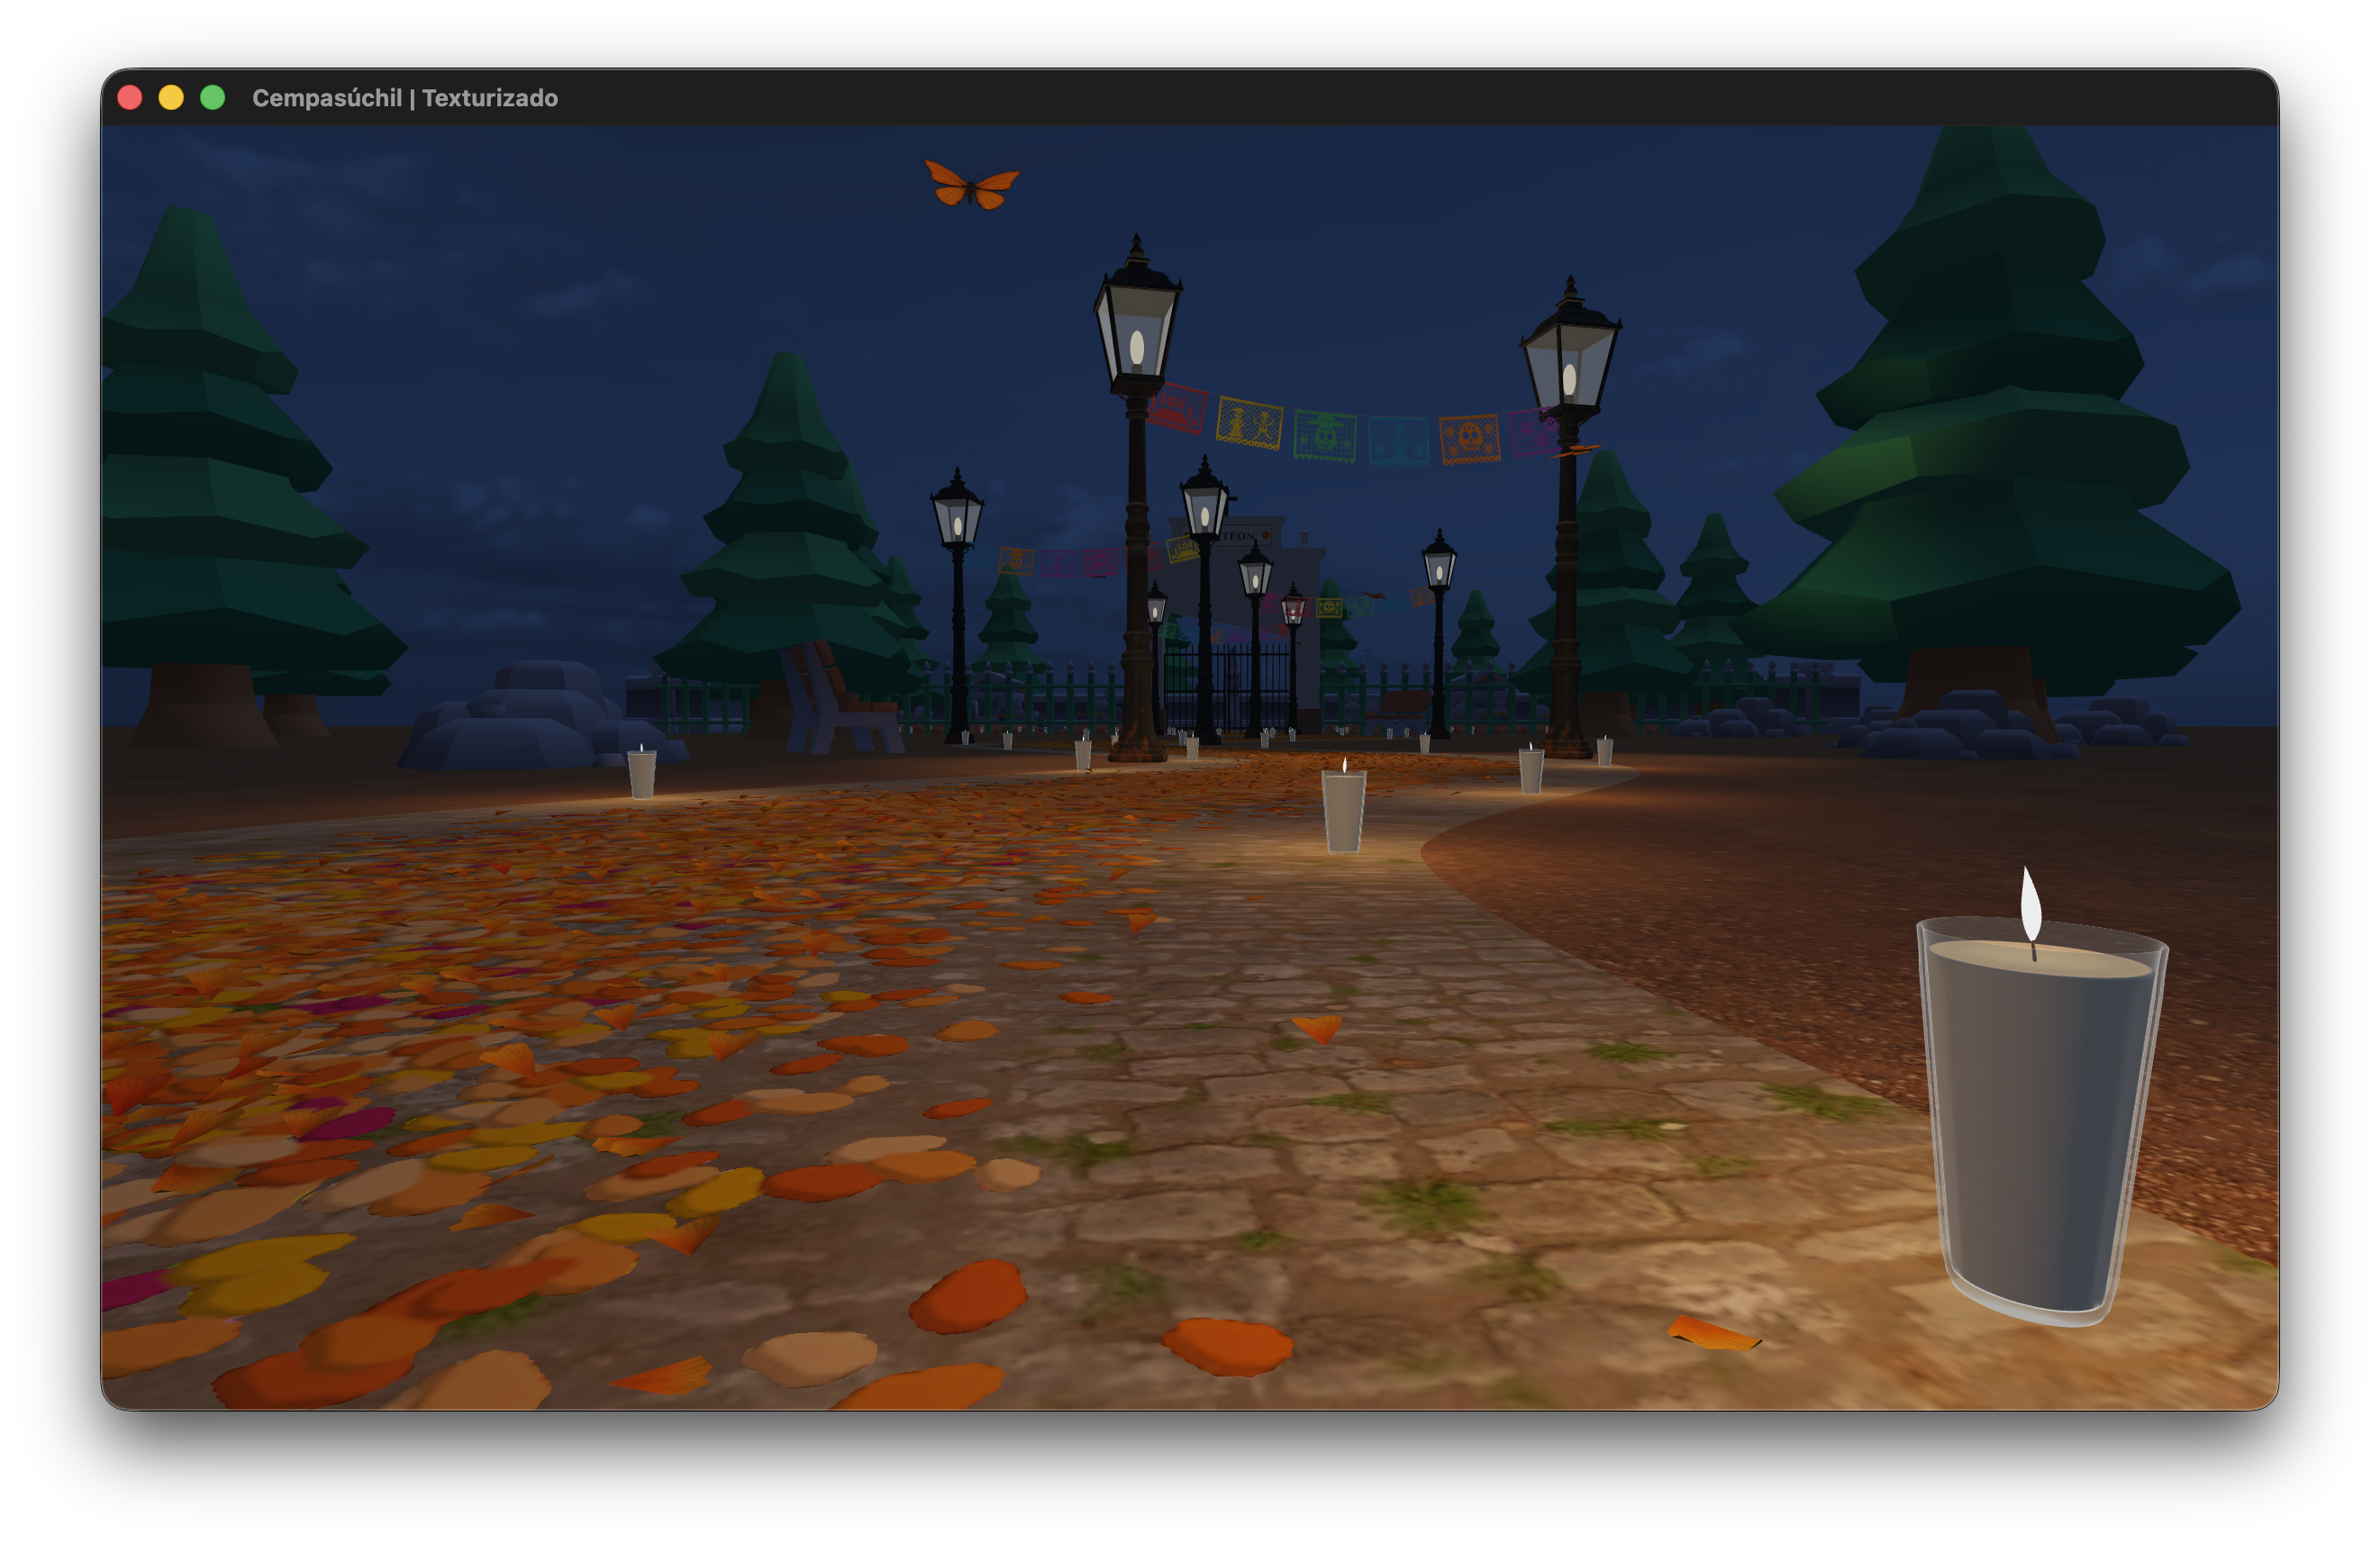
\includegraphics[width=0.85\textwidth]{images/camino.png}
		\caption{Camino empedrado procedural iluminado por faroles y veladoras.}
	\end{figure}
	
	\begin{figure}[H]
		\centering
		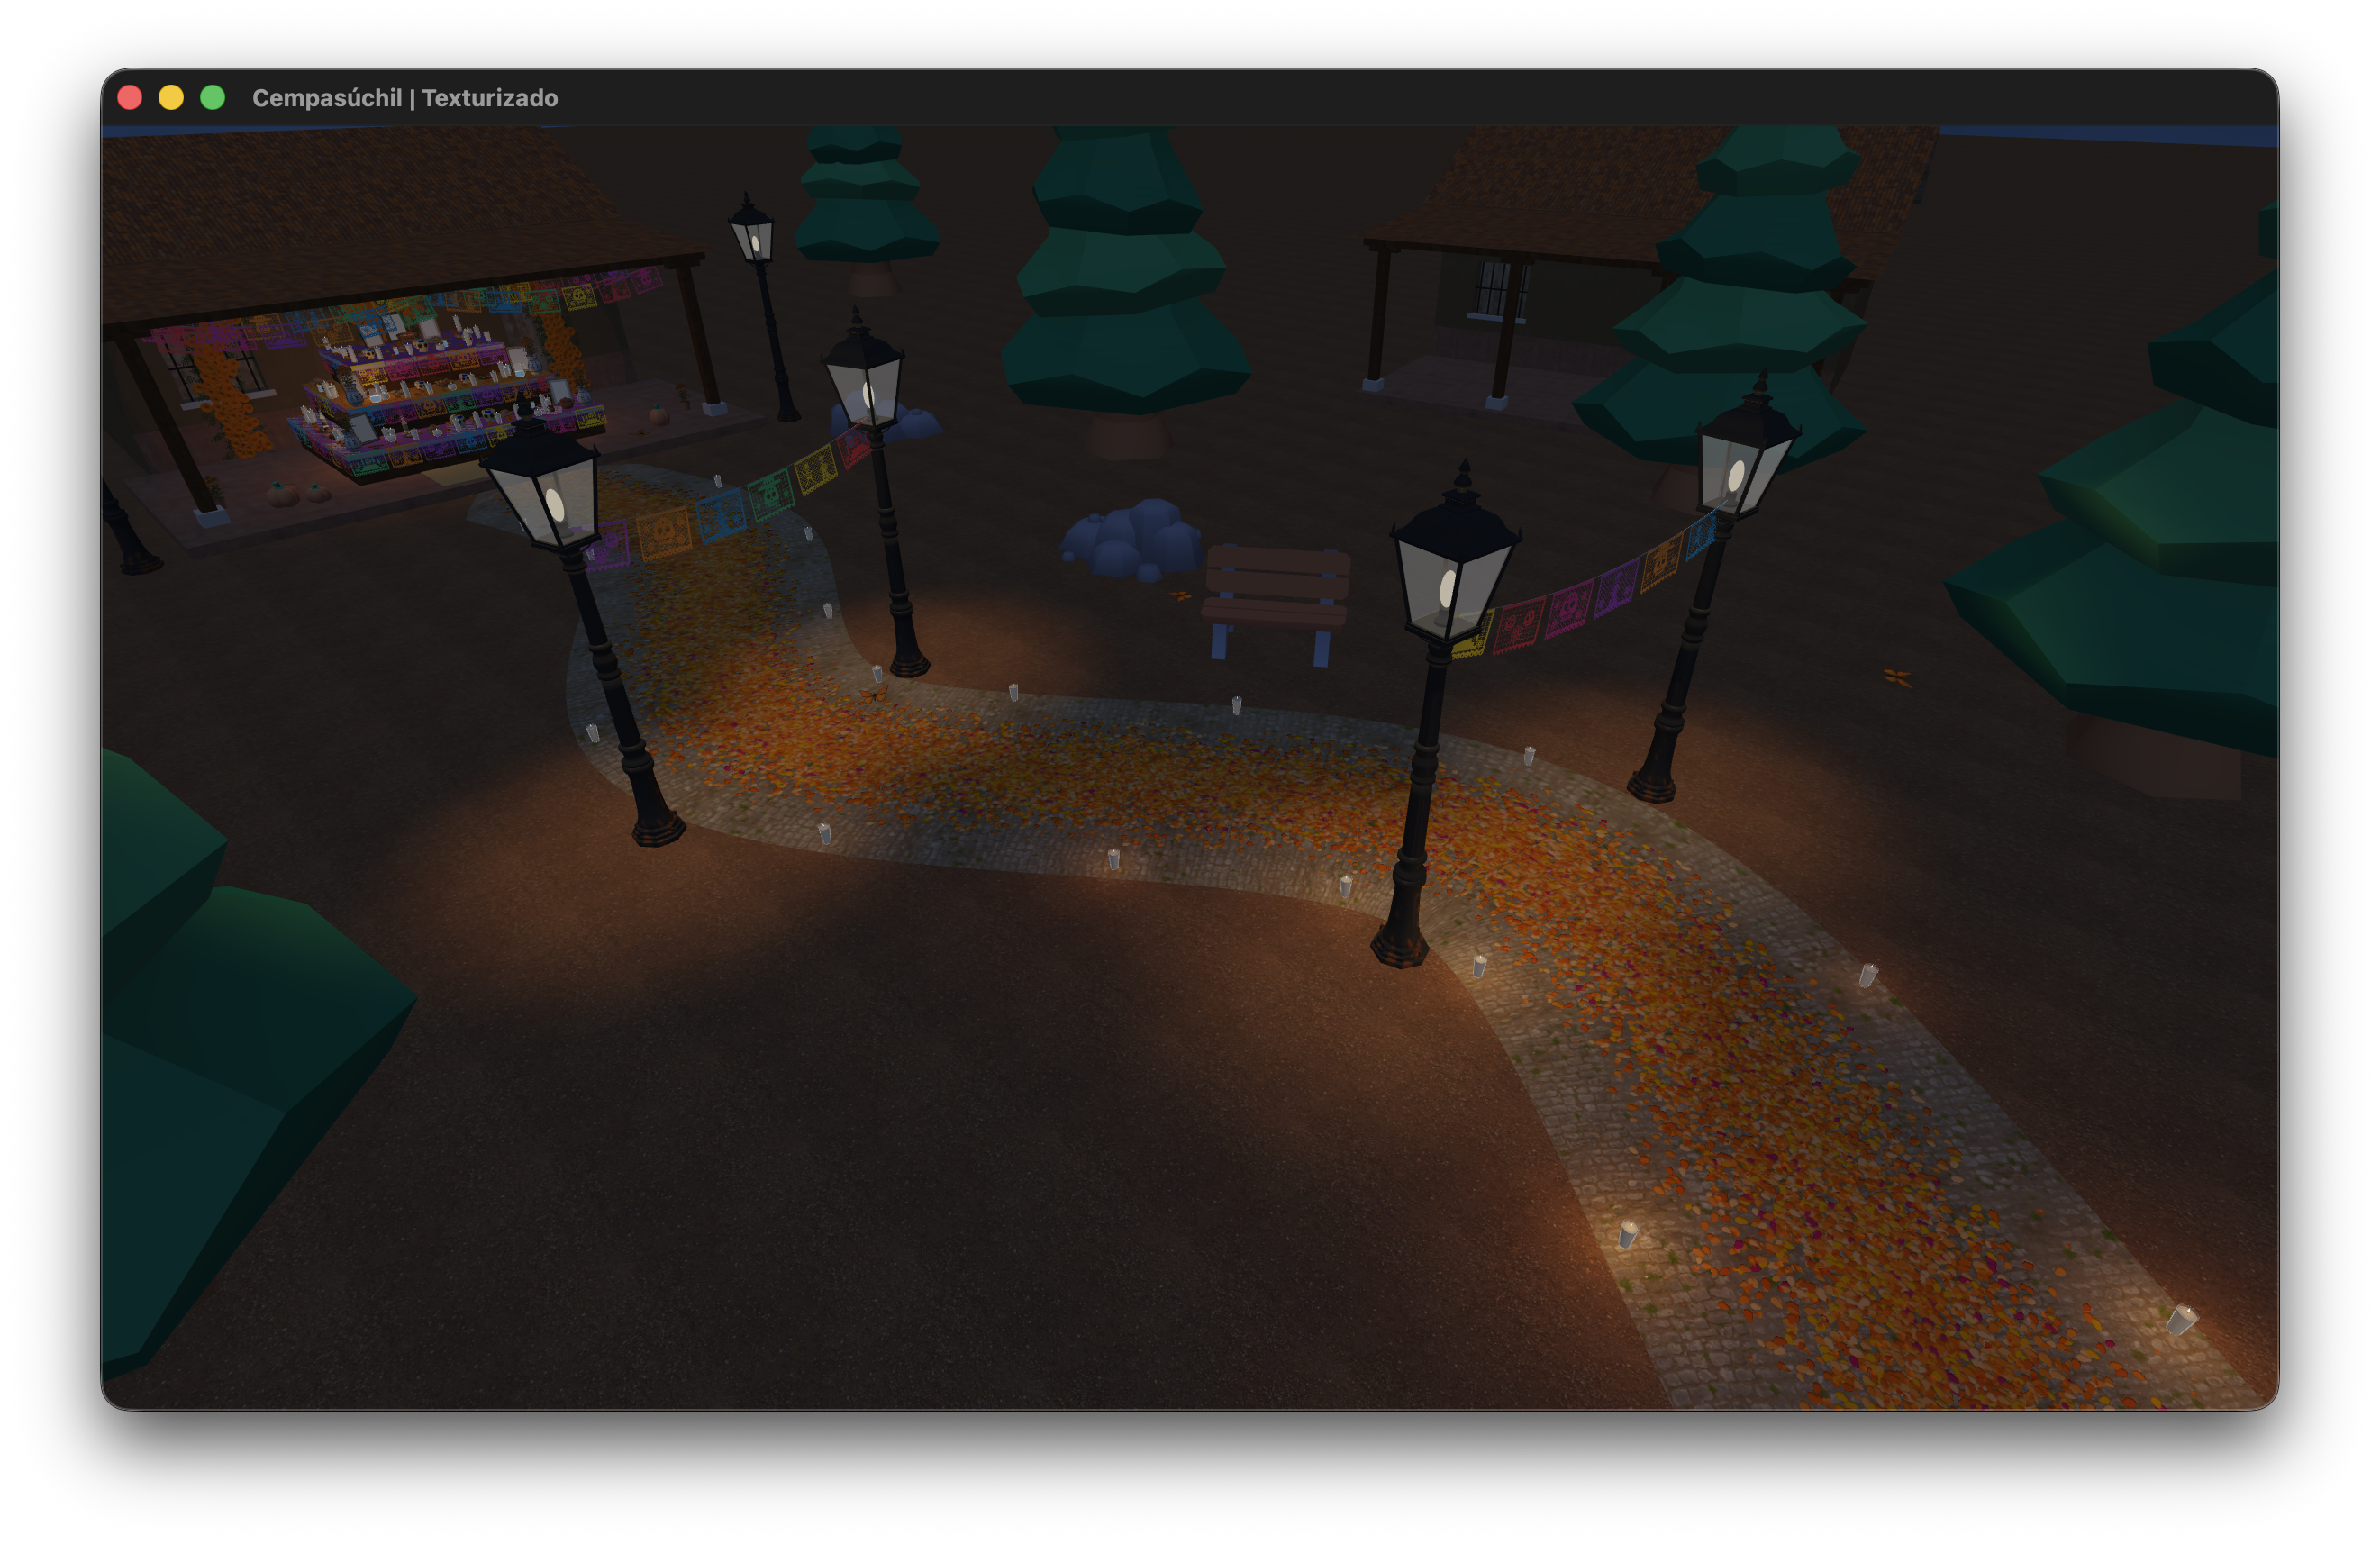
\includegraphics[width=0.85\textwidth]{images/camino-general.png}
		\caption{Vista general del camino iluminado.}
	\end{figure}
	
	
	\section{Compilación y ejecución}
	La ejecución se validó en macOS, Windows físico y Linux. Todas las plataformas requieren una GPU o controlador que proporcione OpenGL 3.3; la presencia de aceleración 3D o DirectX por sí sola no satisface este requisito.
	
	Para optimizar el flujo de trabajo y facilitar la revisión del proyecto, el equipo desarrolló lanzadores nativos para cada sistema operativo. Estos accesos directos automatizan por completo el ciclo de construcción y despliegue, estandarizando el proceso bajo las siguientes características:
	
	\begin{itemize}[leftmargin=1cm]
		\item Configuran y compilan el proyecto a través de CMake estrictamente en modo \texttt{Release}.
		\item Actualizan y sincronizan los directorios de recursos (\texttt{assets} y \texttt{shaders}) hacia el directorio de salida.
		\item Ejecutan la escena automáticamente una vez finalizada la compilación sin procesos en terminal.
		\item Mantienen la consola oculta durante el proceso para ofrecer una experiencia gráfica limpia.
		\item Redirigen y escriben toda la salida técnica, advertencias y diagnósticos en la carpeta \texttt{logs/} ubicada en la raíz del proyecto.
	\end{itemize}
	
	\subsection{Lanzadores por plataforma}
	El repositorio debe encontrarse en una carpeta local con permisos de escritura, pues cada lanzador crea su propio directorio \texttt{build-*}. Los lanzadores no descargan dependencias y se encuentran en \texttt{ejecutables/}.
	
	\subsubsection{macOS}
	Se requiere CMake, las herramientas de línea de comandos de Xcode y soporte del sistema para OpenGL 3.3. Tras clonar o descargar el repositorio, se abre:
	\begin{lstlisting}[style=terminal]
ejecutables/macOS/TexturizadoCempasuchil-0.2.1.app
	\end{lstlisting}
	Por ser una aplicación académica local sin firma, Gatekeeper puede bloquear el primer intento; se debe usar clic derecho, \textbf{Abrir}. El lanzador busca CMake en \texttt{PATH}, Homebrew y la aplicación oficial de CMake, compila en \texttt{build-mac-app/} y conserva el último binario válido si una recompilación posterior falla.

	\subsubsection{Windows}
	Se requiere Windows de 64 bits, un controlador de GPU con OpenGL 3.3, CMake disponible en \texttt{PATH} y Visual Studio Community 2022 o 2026 con la carga \textbf{Desarrollo para el escritorio con C++}, MSVC x64/x86 y un Windows SDK. Después se abre:
	\begin{lstlisting}[style=terminal]
ejecutables\windows\TexturizadoCempasuchil.vbs
	\end{lstlisting}
	VBScript inicia PowerShell sin consola; \texttt{vswhere} selecciona el generador instalado y compila para x64 en \texttt{build-windows-vs17/} o \texttt{build-windows-vs18/}. En Windows ARM64 el ejecutable x64 puede compilarse mediante las herramientas cruzadas, pero la ejecución sigue necesitando un controlador OpenGL compatible.

	\subsubsection{Linux}
	Se requiere CMake, un compilador C++17, OpenGL y los paquetes de desarrollo X11 utilizados por GLFW. En distribuciones basadas en Debian/Ubuntu se puede preparar el entorno con:
	\begin{lstlisting}[style=bashstyle,numbers=none]
sudo apt update
sudo apt install build-essential cmake libgl1-mesa-dev \
    xorg-dev
	\end{lstlisting}
	En Arch Linux se emplean los paquetes equivalentes \texttt{base-devel}, \texttt{cmake}, \texttt{mesa} y \texttt{libx11}. Se marca el archivo \texttt{.desktop} como confiable/ejecutable y se abre, o se ejecuta:
	\begin{lstlisting}[style=bashstyle,numbers=none]
chmod +x ejecutables/linux/iniciar_linux.sh
./ejecutables/linux/iniciar_linux.sh
	\end{lstlisting}

	\subsection{Registros y diagnóstico}
	Los registros de cada plataforma son \path{logs/lanzador-macos.log}, \path{logs/lanzador-windows.log} y \path{logs/lanzador-linux.log}. Los mensajes internos de la escena se almacenan como \path{registro.txt} dentro del directorio de compilación. Si la aplicación informa que no puede crear la ventana, se debe comprobar la versión de OpenGL y actualizar el controlador del fabricante; reinstalar el compilador no corrige una limitación gráfica.
	
	\vspace{0.4cm}
	\textbf{NOTA:} Para mas detalles del funcionamiento interno de la automatización de estos lanzadores, revisar las dependencias exactas de cada sistema o consultar la ubicación de los archivos de registro y diagnóstico, se recomienda leer el archivo \texttt{README.md} ubicado en la ruta \texttt{ejecutables/README.md}.
	
	\section{Resultados y Conclusiones}
	La fase de texturizado e iluminación elevó significativamente el impacto visual y la inmersión del entorno del Día de Muertos. Sin embargo, la implementación del modelo de iluminación híbrida presentó un reto importante de rendimiento para el equipo. Al integrar las fuentes de luz dinámica, detectamos cuellos de botella severos debido a que algunos modelos exportados desde Blender poseían una densidad poligonal excesiva; el motor gráfico estaba calculando la iluminación por fragmento sobre una cantidad innecesaria de triángulos, saturando el procesamiento. La solución implementada fue optimizar estos modelos, reduciendo drásticamente su conteo de triángulos (retopología y diezmado) pero conservando una apariencia visual prácticamente idéntica a la original gracias al detalle aportado por los mapas de normales.
	
	El uso de texturas PBR elaboradas procedimentalmente, acoplado al cálculo de normales derivado directamente en el \textit{fragment shader}, demostró un excelente equilibrio entre calidad fotográfica y optimización algorítmica. Asimismo, el diseño arquitectónico multiplataforma fue crucial para superar con éxito barreras técnicas de librerías nativas, sistemas de archivos, repositorios e interfaces de alta resolución. 
	
	El correcto mapeo alfa para reducir polígonos (como en la alfombra de pétalos), la optimización geométrica de las mallas y el sistema de refracción simulada permiten afirmar que la entrega cumple satisfactoriamente con los parámetros visuales propuestos. Para la fase final, el entorno técnico robusto y optimizado construido hasta el momento servirá como base ideal para integrar de forma fluida sistemas de partículas y animaciones.
	
	\section{Referencias}
	\begin{itemize}[leftmargin=*]
		\item Blender Foundation. (2026). \textit{Blender 5.2}. \url{https://www.blender.org/}
		\item Khronos Group. (2021). \textit{glTF 2.0 Specification}. \url{https://registry.khronos.org/glTF/specs/2.0/glTF-2.0.html}
		\item Khronos Group. (2010). \textit{OpenGL 3.3 Core Profile Specification}. \url{https://registry.khronos.org/OpenGL/specs/gl/glspec33.core.pdf}
		\item Kitware. (2026). \textit{CMake Documentation}. \url{https://cmake.org/documentation/}
		\item nothings/stb. (2025). \textit{stb\_image 2.30}. \url{https://github.com/nothings/stb}
		\item GLFW. (2026). \textit{GLFW Documentation}. \url{https://www.glfw.org/documentation.html}
	\end{itemize}
\end{document}
